% 原书印刷页 24--33。公式与算法均为原生可编辑 LaTeX。
\begin{example}{3.5}
\sourcepage{24}
考虑例~3.2 中的问题：对于 $\mathbf{f}:\R^n\to\R^n$，求解 $\mathbf{f}(\mathbf{x}^*)=\mathbf{0}$。若用 Newton--Raphson 法求解这个问题，其典型迭代步为
\[
  \text{求解 }\mathbf{J}(\mathbf{x})\mathbf{h}_{\mathrm{nr}}=-\mathbf{f}(\mathbf{x});\qquad \mathbf{x}:=\mathbf{x}+\mathbf{h}_{\mathrm{nr}}.
\]
把 Gauss--Newton 法用于极小化 $F(\mathbf{x})=\tfrac12 \mathbf{f}(\mathbf{x})^{\T}\mathbf{f}(\mathbf{x})$ 时，其典型步骤为
\[
  \text{求解 }\bigl(\mathbf{J}(\mathbf{x})^{\T}\mathbf{J}(\mathbf{x})\bigr)\mathbf{h}_{\mathrm{gn}}=-\mathbf{J}(\mathbf{x})^{\T}\mathbf{f}(\mathbf{x});
  \qquad \mathbf{x}:=\mathbf{x}+\mathbf{h}_{\mathrm{gn}}.
\]
注意，$\mathbf{J}(\mathbf{x})$ 是方阵，并且我们假设它非奇异。因此 $(\mathbf{J}(\mathbf{x})^{\T})^{-1}$ 存在，进而有 $\mathbf{h}_{\mathrm{gn}}=\mathbf{h}_{\mathrm{nr}}$。所以，把 Gauss--Newton 法用于例~3.2 中的 Powell 问题时，会遇到该例讨论 Newton--Raphson 法时所遇到的同样困难。
\end{example}

这些例子表明，无论是否采用线搜索，Gauss--Newton 法都有可能失败。不过，在许多应用中它的表现相当好，尽管它通常只有线性收敛性，而实现了二阶导数的 Newton 法具有二次收敛性。

第~3.2 节和第~3.3 节给出两种全局性能更好的方法，第~3.4 节则对第一种方法作一些修改，以获得超线性的最终收敛速度。

\section{Levenberg--Marquardt 法}\label{sec:lm}
Levenberg（1944）以及后来的 Marquardt（1963）提出采用阻尼 Gauss--Newton 法，参见第~2.4 节。步 $\mathbf{h}_{\mathrm{lm}}$ 由式~\eqref{eq:3.9} 的以下修改来定义：
\begin{equation}
  (\mathbf{J}^{\T}\mathbf{J}+\mu \mathbf{I})\mathbf{h}_{\mathrm{lm}}=-\mathbf{g},
  \qquad \mathbf{g}=\mathbf{J}^{\T}\mathbf{f},\quad \mu\geq0.
  \tag{3.13}\label{eq:3.13}
\end{equation}
这里，$\mathbf{J}=\mathbf{J}(\mathbf{x})$，$\mathbf{f}=\mathbf{f}(\mathbf{x})$。阻尼参数 $\mu$ 有以下几方面作用：
\begin{enumerate}[label=\alph*),leftmargin=2.2em]
\item 对所有 $\mu>0$，系数矩阵都是正定的，这保证 $\mathbf{h}_{\mathrm{lm}}$ 是下降方向，参见式~\eqref{eq:3.10}。
\sourcepage{25}
\item 当 $\mu$ 很大时，有
\[
  \mathbf{h}_{\mathrm{lm}}\simeq-\frac1\mu \mathbf{g}=-\frac1\mu \mathbf{F}'(\mathbf{x}),
\]
即沿最速下降方向走一个短步。当当前迭代点离解较远时，这是有益的。
\item 若 $\mu$ 很小，则 $\mathbf{h}_{\mathrm{lm}}\simeq \mathbf{h}_{\mathrm{gn}}$。在迭代的最后阶段，即 $\mathbf{x}$ 接近 $\mathbf{x}^*$ 时，这是一个很好的步。若 $F(\mathbf{x}^*)=0$（或非常小），则可以获得（近乎）二次的最终收敛速度。
\end{enumerate}
因此，阻尼参数既影响步的方向，也影响步的大小，这使我们得以构造一种不需要专门线搜索的方法。

初始 $\mu$ 值的选择应与 $\mathbf{A}_0=\mathbf{J}(\mathbf{x}_0)^{\T}\mathbf{J}(\mathbf{x}_0)$ 中元素的大小有关，例如令
\begin{equation}
  \mu_0=\tau\cdot\max_i\{a_{ii}^{(0)}\},
  \tag{3.14}\label{eq:3.14}
\end{equation}
其中 $\tau$ 由用户选择。\footnote[3]{算法对 $\tau$ 的选择不是很敏感。不过，按照经验，若认为 $\mathbf{x}_0$ 是 $\mathbf{x}^*$ 的良好近似，就应取较小的值，例如 $\tau=10^{-6}$；否则可取 $\tau=10^{-3}$，甚至 $\tau=1$。}迭代过程中可以按第~2.4 节所述更新 $\mu$ 的大小。更新由增益比控制：
\[
  \varrho=\frac{F(\mathbf{x})-F(\mathbf{x}+\mathbf{h}_{\mathrm{lm}})}{L(\mathbf{0})-L(\mathbf{h}_{\mathrm{lm}})},
\]
其中分母是线性模型~\eqref{eq:3.7b} 预测的增益，
\[
\begin{aligned}
 L(\mathbf{0})-L(\mathbf{h}_{\mathrm{lm}})
  &=-\mathbf{h}_{\mathrm{lm}}^{\T}\mathbf{J}^{\T}\mathbf{f}
      -\tfrac12\mathbf{h}_{\mathrm{lm}}^{\T}\mathbf{J}^{\T}\mathbf{J}\mathbf{h}_{\mathrm{lm}}\\
  &=-\tfrac12\mathbf{h}_{\mathrm{lm}}^{\T}
      \bigl(2\mathbf{g}+(\mathbf{J}^{\T}\mathbf{J}+\mu \mathbf{I}-\mu \mathbf{I})\mathbf{h}_{\mathrm{lm}}\bigr)\\
  &=\tfrac12\mathbf{h}_{\mathrm{lm}}^{\T}(\mu \mathbf{h}_{\mathrm{lm}}-\mathbf{g}).
\end{aligned}
\]
注意，$\mathbf{h}_{\mathrm{lm}}^{\T}\mathbf{h}_{\mathrm{lm}}$ 和 $-\mathbf{h}_{\mathrm{lm}}^{\T}\mathbf{g}$ 都为正，因此 $L(\mathbf{0})-L(\mathbf{h}_{\mathrm{lm}})$ 保证为正。

较大的 $\varrho$ 值表示 $L(\mathbf{h}_{\mathrm{lm}})$ 是 $F(\mathbf{x}+\mathbf{h}_{\mathrm{lm}})$ 的良好近似，这时可以减小 $\mu$，使下一个 Levenberg--Marquardt
\sourcepage{26}
步更接近 Gauss--Newton 步。若 $\varrho$ 很小（甚至为负），则 $L(\mathbf{h}_{\mathrm{lm}})$ 是一个较差的近似，应增大 $\mu$，一方面使方向更接近最速下降方向，另一方面缩短步长。有多种方式可以同时达到这两个目的，参见第~\pageref{src:14}~页和下面的例~3.7。

算法的停止准则应体现如下事实：在全局极小点处有 $\mathbf{F}'(\mathbf{x}^*)=\mathbf{g}(\mathbf{x}^*)=\mathbf{0}$。因此可以采用
\begin{equation}
  \norm{\mathbf{g}}_{\infty}\leq\varepsilon_1,
  \tag{3.15a}\label{eq:3.15a}
\end{equation}
其中 $\varepsilon_1$ 是用户选定的一个很小的正数。另一个有用的准则是，当 $\mathbf{x}$ 的变化很小时停止：
\begin{equation}
  \norm{\mathbf{x}_{\mathrm{new}}-\mathbf{x}}\leq\varepsilon_2(\norm{\mathbf{x}}+\varepsilon_2).
  \tag{3.15b}\label{eq:3.15b}
\end{equation}
这个表达式使步长准则从 $\norm{\mathbf{x}}$ 很大时的相对步长 $\varepsilon_2$，平滑过渡到 $\mathbf{x}$ 接近 $\mathbf{0}$ 时的绝对步长 $\varepsilon_2^2$。最后，与所有迭代过程一样，需要设置防止无限循环的保护条件：
\begin{equation}
  k\geq k_{\max}.
  \tag{3.15c}\label{eq:3.15c}
\end{equation}
$\varepsilon_2$ 和 $k_{\max}$ 也由用户选择。

例如，若 $\varepsilon_1$ 取得太小，以至舍入误差的影响很大，最后两个准则就会发挥作用。这种情形通常表现为 $F$ 的实际增益与线性模型~\eqref{eq:3.7b} 预测的增益吻合较差，因而每一步都要增大 $\mu$。采用增大 $\mu$ 的策略~\eqref{eq:2.21}，这时 $\mu$ 会迅速增长，使 $\norm{\mathbf{h}_{\mathrm{lm}}}$ 变得很小，于是过程将由准则~\eqref{eq:3.15b} 停止。

算法概括如下。

% 原版算法为印刷页 27 页首浮动块；此处紧随其引导句，以免割裂例 3.6。
\needspace{24\baselineskip}
\sourcepage{27}
\begin{algorithmbox}{3.16}{Levenberg--Marquardt 法}
\begin{tabbing}
\hspace{1.2em}\=\hspace{1.2em}\=\hspace{1.2em}\=\hspace{1.2em}\=\hspace{1.2em}\=\kill
\textbf{begin}\\
\> $k:=0;\quad\nu:=2;\quad \mathbf{x}:=\mathbf{x}_0$\\
\> $\mathbf{A}:=\mathbf{J}(\mathbf{x})^{\T}\mathbf{J}(\mathbf{x});\quad \mathbf{g}:=\mathbf{J}(\mathbf{x})^{\T}\mathbf{f}(\mathbf{x})$\\
\> $\mathit{found}:=(\norm{\mathbf{g}}_{\infty}\leq\varepsilon_1);\quad
       \mu:=\tau*\max\{a_{ii}\}$\\
\> \textbf{while} (\textbf{not} $\mathit{found}$) \textbf{and} $(k<k_{\max})$\\
\>\> $k:=k+1;$\quad 求解 $(\mathbf{A}+\mu \mathbf{I})\mathbf{h}_{\mathrm{lm}}=-\mathbf{g}$\\
\>\> \textbf{if} $\norm{\mathbf{h}_{\mathrm{lm}}}\leq\varepsilon_2(\norm{\mathbf{x}}+\varepsilon_2)$\\
\>\>\> $\mathit{found}:=\mathbf{true}$\\
\>\> \textbf{else}\\
\>\>\> $\mathbf{x}_{\mathrm{new}}:=\mathbf{x}+\mathbf{h}_{\mathrm{lm}}$\\
\>\>\> $\varrho:=(F(\mathbf{x})-F(\mathbf{x}_{\mathrm{new}}))/(L(\mathbf{0})-L(\mathbf{h}_{\mathrm{lm}}))$\\
\>\>\> \textbf{if} $\varrho>0$\qquad\qquad $\{\text{该步可接受}\}$\\
\>\>\>\> $\mathbf{x}:=\mathbf{x}_{\mathrm{new}}$\\
\>\>\>\> $\mathbf{A}:=\mathbf{J}(\mathbf{x})^{\T}\mathbf{J}(\mathbf{x});\quad \mathbf{g}:=\mathbf{J}(\mathbf{x})^{\T}\mathbf{f}(\mathbf{x})$\\
\>\>\>\> $\mathit{found}:=(\norm{\mathbf{g}}_{\infty}\leq\varepsilon_1)$\\
\>\>\>\> $\mu:=\mu*\max\{\tfrac13,1-(2\varrho-1)^3\};\quad\nu:=2$\\
\>\>\> \textbf{else}\\
\>\>\>\> $\mu:=\mu*\nu;\quad\nu:=2*\nu$\\
\textbf{end}
\end{tabbing}
\end{algorithmbox}

\begin{example}{3.6}
比较式~\eqref{eq:3.9} 和正规方程~\eqref{eq:3.5}，可知 $\mathbf{h}_{\mathrm{gn}}$ 就是线性问题
\[
  \mathbf{f}(\mathbf{x})+\mathbf{J}(\mathbf{x})\mathbf{h}\simeq\mathbf{0}
\]
的最小二乘解。类似地，L-M 方程~\eqref{eq:3.13} 是线性问题
\[
  \begin{bmatrix}\mathbf{f}(\mathbf{x})\\\mathbf{0}\end{bmatrix}
  +\begin{bmatrix}\mathbf{J}(\mathbf{x})\\\sqrt\mu \mathbf{I}\end{bmatrix}\mathbf{h}\simeq\mathbf{0}
\]
的正规方程。如例~3.1 所述，通过正交变换可以求得最精确的解。不过，解 $\mathbf{h}_{\mathrm{lm}}$ 只是迭代过程中的一个步，不必算得非常精确，而通过正规方程求解的计算代价较低，因此通常采用这种方法。
\end{example}

\begin{example}{3.7}
我们把算法~3.16 用于例~1.1 和例~3.4 中的数据拟合问题。图~1.1 表明，$x_1$ 和 $x_2$ 都是负的，且 $M(\mathbf{x}^*,0)\simeq0$。初始点 $\mathbf{x}_0=[-1,-2,1,-1]^{\T}$ 满足这些条件。此外，在给出 $\mu_0$ 的式~\eqref{eq:3.14} 中取 $\tau=10^{-3}$，并在式~(3.15)
\sourcepage{28}
给出的停止准则中取 $\varepsilon_1=\varepsilon_2=10^{-8}$、$k_{\max}=200$。算法在迭代了 $62$ 步之后停止，得到 $\mathbf{x}\simeq[-4,-5,4,-4]^{\T}$。下面的图显示了其表现；注意纵坐标采用对数刻度。

这个问题是不相容的，因此可以预期最终呈线性收敛。最后 $7$ 个迭代步却显示出好得多的（超线性）收敛性。原因在于 $f_i''(\mathbf{x})$ 是随 $t_i$ 缓慢变化的函数，而 $f_i(\mathbf{x}^*)$ 的符号具有“随机性”，因此它们对式~\eqref{eq:3.12} 中“被忽略项”的贡献几乎相互抵消。这种情形在许多数据拟合应用中都会出现。

\begin{figure}[H]
\centering
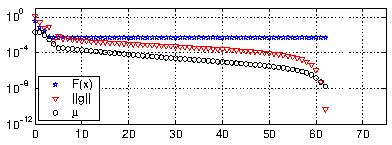
\includegraphics[width=0.72\linewidth]{assets/figures/fig-3-2a.pdf}
\begingroup
\setcounter{figure}{1}
\renewcommand{\thefigure}{3.2a}
\renewcommand{\theHfigure}{3.2a}
\caption{L-M 法用于例~1.1 中的拟合问题。}\label{fig:3.2a}\label{fig:3.2}
\endgroup
\end{figure}

为作比较，图~\ref{fig:3.2b} 给出了采用更新策略~\eqref{eq:2.20} 时的表现。从第 $5$ 步到第 $68$ 步，每次 $\mu$ 减小后都立即随之增大，梯度的范数也呈现出起伏不平的变化。这使收敛变慢，但最后阶段与图~\ref{fig:3.2a} 相同。

\begin{figure}[H]
\centering
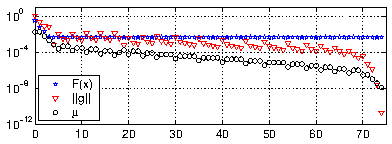
\includegraphics[width=0.72\linewidth]{assets/figures/fig-3-2b.pdf}
\begingroup
\setcounter{figure}{1}
\renewcommand{\thefigure}{3.2b}
\renewcommand{\theHfigure}{3.2b}
\caption{采用更新策略~\eqref{eq:2.20} 时的表现。}\label{fig:3.2b}
\endgroup
\end{figure}
\setcounter{figure}{2}
\end{example}

\begin{example}{3.8}
图~\ref{fig:3.3} 展示了将算法~3.16 用于例~3.2 和例~3.5 中 Powell 问题时的表现。初始点为 $\mathbf{x}_0=[3,1]^{\T}$，$\mu_0$ 由式~\eqref{eq:3.14} 中的 $\tau=1$ 给出，在停止准则~(3.15) 中取 $\varepsilon_1=\varepsilon_2=10^{-15}$、$k_{\max}=100$。

\sourcepage{29}
\begin{figure}[H]
\centering
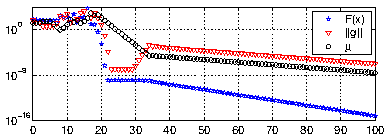
\includegraphics[width=0.72\linewidth]{assets/figures/fig-3-3.pdf}
\setcounter{figure}{2}
\caption{L-M 法用于 Powell 问题。}\label{fig:3.3}
\end{figure}

迭代在第 $22$ 步至第 $30$ 步之间似乎停滞了。这是 Jacobian 矩阵（几乎）奇异所造成的。此后似乎呈线性收敛。迭代由“保护条件”停止，停止点为 $\mathbf{x}=[-3.82\mathrm{e}{-08},-1.38\mathrm{e}{-03}]^{\T}$。这比在例~3.2 中得到的结果更接近 $\mathbf{x}^*=\mathbf{0}$，但我们希望还能做得更好，参见例~3.10 和例~3.17。
\end{example}

\section{Powell 狗腿法}\label{sec:dogleg}
与 Levenberg--Marquardt 法一样，这种方法也采用 Gauss--Newton 方向与最速下降方向的组合。不过，这里的控制是显式地通过信赖域的半径进行的，参见第~2.4 节。这一算法之所以与 Powell 的名字相联系，是因为他提出了求取式~\eqref{eq:2.23} 所定义的 $\mathbf{h}_{\mathrm{tr}}$ 的近似的方法。

给定 $\mathbf{f}:\R^n\to\R^m$。在当前迭代点 $\mathbf{x}$ 处，Gauss--Newton 步 $\mathbf{h}_{\mathrm{gn}}$ 是线性系统
\begin{equation}
  \mathbf{J}(\mathbf{x})\mathbf{h}\simeq-\mathbf{f}(\mathbf{x})
  \tag{3.17}\label{eq:3.17}
\end{equation}
的最小二乘解。它可以通过求解正规方程
\begin{equation}
  \bigl(\mathbf{J}(\mathbf{x})^{\T}\mathbf{J}(\mathbf{x})\bigr)\mathbf{h}_{\mathrm{gn}}=-\mathbf{J}(\mathbf{x})^{\T}\mathbf{f}(\mathbf{x})
  \tag{3.18a}\label{eq:3.18a}
\end{equation}
来计算。

最速下降方向由下式给出：
\begin{equation}
  \mathbf{h}_{\mathrm{sd}}=-\mathbf{g}=-\mathbf{J}(\mathbf{x})^{\T}\mathbf{f}(\mathbf{x}).
  \tag{3.18b}\label{eq:3.18b}
\end{equation}
这是一个方向，而非一个步。为确定应沿此方向走多远，我们考察线性模型
\sourcepage{30}
\[
\begin{aligned}
  &\mathbf{f}(\mathbf{x}+\alpha \mathbf{h}_{\mathrm{sd}})\simeq \mathbf{f}(\mathbf{x})+\alpha \mathbf{J}(\mathbf{x})\mathbf{h}_{\mathrm{sd}}\\
  &\Downarrow\\
  &F(\mathbf{x}+\alpha \mathbf{h}_{\mathrm{sd}})
     \simeq\tfrac12\norm{\mathbf{f}(\mathbf{x})+\alpha \mathbf{J}(\mathbf{x})\mathbf{h}_{\mathrm{sd}}}^2\\
  &\hphantom{F(\mathbf{x}+\alpha \mathbf{h}_{\mathrm{sd}})}
     =F(\mathbf{x})+\alpha \mathbf{h}_{\mathrm{sd}}^{\T}\mathbf{J}(\mathbf{x})^{\T}\mathbf{f}(\mathbf{x})
           +\tfrac12\alpha^2\norm{\mathbf{J}(\mathbf{x})\mathbf{h}_{\mathrm{sd}}}^2.
\end{aligned}
\]
这个关于 $\alpha$ 的函数在下列值处达到最小：
\begin{equation}
  \alpha=-\frac{\mathbf{h}_{\mathrm{sd}}^{\T}\mathbf{J}(\mathbf{x})^{\T}\mathbf{f}(\mathbf{x})}
                 {\norm{\mathbf{J}(\mathbf{x})\mathbf{h}_{\mathrm{sd}}}^2}
         =\frac{\norm{\mathbf{g}}^2}{\norm{\mathbf{J}(\mathbf{x})\mathbf{g}}^2}.
  \tag{3.19}\label{eq:3.19}
\end{equation}
现在，从当前点 $\mathbf{x}$ 出发的步有两个候选：$\mathbf{a}=\alpha \mathbf{h}_{\mathrm{sd}}$ 和 $\mathbf{b}=\mathbf{h}_{\mathrm{gn}}$。当信赖域半径为 $\Delta$ 时，Powell 提出采用以下策略选择步。策略中的最后一种情形如图~\ref{fig:3.4} 所示。
\begin{equation}
\begin{aligned}
 &\textbf{if}\quad \norm{\mathbf{h}_{\mathrm{gn}}}\leq\Delta\\
 &\qquad \mathbf{h}_{\mathrm{dl}}:=\mathbf{h}_{\mathrm{gn}}\\
 &\textbf{elseif}\quad \norm{\alpha \mathbf{h}_{\mathrm{sd}}}\geq\Delta\\
 &\qquad \mathbf{h}_{\mathrm{dl}}:=(\Delta/\norm{\mathbf{h}_{\mathrm{sd}}})\mathbf{h}_{\mathrm{sd}}\\
 &\textbf{else}\\
 &\qquad \mathbf{h}_{\mathrm{dl}}:=\alpha \mathbf{h}_{\mathrm{sd}}
                     +\beta(\mathbf{h}_{\mathrm{gn}}-\alpha \mathbf{h}_{\mathrm{sd}})\\
 &\qquad \text{其中选择 }\beta\text{ 使得 }\norm{\mathbf{h}_{\mathrm{dl}}}=\Delta.
\end{aligned}
\tag{3.20a}\label{eq:3.20a}
\end{equation}

\begin{figure}[H]
\centering
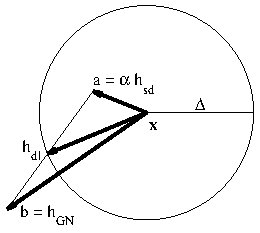
\includegraphics[width=0.44\linewidth]{assets/figures/fig-3-4.pdf}
\setcounter{figure}{3}
\caption{信赖域与狗腿步。\protect\footnotemark[4]}\label{fig:3.4}
\end{figure}
\footnotetext[4]{“狗腿”（Dog Leg）这一名称来自高尔夫球：在“狗腿洞”中，球道的形状就像从 $\mathbf{x}$（发球点）经过 $\mathbf{a}$ 的端点，再到 $\mathbf{h}_{\mathrm{dl}}$ 的端点（球洞）的折线。Powell 是一位热衷高尔夫球的人！}

\needspace{4\baselineskip}
\sourcepage{31}
令 $\mathbf{a}$、$\mathbf{b}$ 如上所定义，并令 $c=\mathbf{a}^{\T}(\mathbf{b}-\mathbf{a})$，则可写成
\[
 \psi(\beta)\equiv\norm{\mathbf{a}+\beta(\mathbf{b}-\mathbf{a})}^2-\Delta^2
 =\norm{\mathbf{b}-\mathbf{a}}^2\beta^2+2c\beta+\norm{\mathbf{a}}^2-\Delta^2.
\]
我们要找这个二次多项式的一个根。注意，$\beta\to-\infty$ 时 $\psi\to+\infty$；$\psi(0)=\norm{\mathbf{a}}^2-\Delta^2<0$；$\psi(1)=\norm{\mathbf{h}_{\mathrm{gn}}}^2-\Delta^2>0$。因此，$\psi$ 有一个负根和一个位于 $]0,1[$ 内的根。我们要找后者，最精确的计算方式为
\begin{equation}
\begin{aligned}
 &\textbf{if}\quad c\leq0\\
 &\quad\beta=
 \frac{-c+\sqrt{c^2+\norm{\mathbf{b}-\mathbf{a}}^2(\Delta^2-\norm{\mathbf{a}}^2)}}{\norm{\mathbf{b}-\mathbf{a}}^2}\\
 &\textbf{else}\\
 &\quad\beta=
 \frac{\Delta^2-\norm{\mathbf{a}}^2}
      {c+\sqrt{c^2+\norm{\mathbf{b}-\mathbf{a}}^2(\Delta^2-\norm{\mathbf{a}}^2)}}.
\end{aligned}
\tag{3.20b}\label{eq:3.20b}
\end{equation}
与 L-M 法一样，可以用增益比
\[
  \varrho=\bigl(F(\mathbf{x})-F(\mathbf{x}+\mathbf{h}_{\mathrm{dl}})\bigr)
            /\bigl(L(\mathbf{0})-L(\mathbf{h}_{\mathrm{dl}})\bigr)
\]
来监控迭代。这里，$L$ 仍然是线性模型
\[
  L(\mathbf{h})=\tfrac12\norm{\mathbf{f}(\mathbf{x})+\mathbf{J}(\mathbf{x})\mathbf{h}}^2.
\]
在 L-M 法中，我们用 $\varrho$ 控制阻尼参数的大小；这里则用它控制信赖域的半径 $\Delta$。较大的 $\varrho$ 值表示线性模型很好。这时可以增大 $\Delta$，从而走更长的步，且这些步更接近 Gauss--Newton 方向。若 $\varrho$ 很小（甚至为负），则减小 $\Delta$，这意味着步更短、方向更接近最速下降方向。下面概括这一算法。作如下说明。
\begin{enumerate}[label=$\arabic*^{\circ}$,leftmargin=2.2em]
\item 初始化。$\mathbf{x}_0$ 和 $\Delta_0$ 应由用户提供。
\item 采用停止准则~(3.15)，并补充 $\norm{\mathbf{f}(\mathbf{x})}_{\infty}\leq\varepsilon_3$，以体现当 $m=n$、即问题为非线性方程组时有 $\mathbf{f}(\mathbf{x}^*)=\mathbf{0}$。
\item 若 $m=n$，则将“$\simeq$”换成“$=$”，参见式~\eqref{eq:3.6}，并且不再绕道求解正规方程~\eqref{eq:3.18a}，参见例~3.9。
\end{enumerate}

\needspace{24\baselineskip}
\sourcepage{32}
\begin{algorithmbox}{3.21}{狗腿法}
\begin{tabbing}
\hspace{1.15em}\=\hspace{1.15em}\=\hspace{1.15em}\=\hspace{1.15em}\=\hspace{1.15em}\=\kill
\textbf{begin}\\
\> $k:=0;\quad \mathbf{x}:=\mathbf{x}_0;\quad\Delta:=\Delta_0;\quad \mathbf{g}:=\mathbf{J}(\mathbf{x})^{\T}\mathbf{f}(\mathbf{x})$\quad $\{1^{\circ}\}$\\
\> $\mathit{found}:=(\norm{\mathbf{f}(\mathbf{x})}_{\infty}\leq\varepsilon_3)$ \textbf{or}
   $(\norm{\mathbf{g}}_{\infty}\leq\varepsilon_1)$\quad $\{2^{\circ}\}$\\
\> \textbf{while} (\textbf{not} $\mathit{found}$) \textbf{and} $(k<k_{\max})$\\
\>\> $k:=k+1;$\quad 按式~\eqref{eq:3.19} 计算 $\alpha$\\
\>\> $\mathbf{h}_{\mathrm{sd}}:=-\alpha \mathbf{g};$\quad 求解 $\mathbf{J}(\mathbf{x})\mathbf{h}_{\mathrm{gn}}\simeq-\mathbf{f}(\mathbf{x})$\quad $\{3^{\circ}\}$\\
\>\> 按式~(3.20) 计算 $\mathbf{h}_{\mathrm{dl}}$\\
\>\> \textbf{if} $\norm{\mathbf{h}_{\mathrm{dl}}}\leq\varepsilon_2(\norm{\mathbf{x}}+\varepsilon_2)$\\
\>\>\> $\mathit{found}:=\mathbf{true}$\\
\>\> \textbf{else}\\
\>\>\> $\mathbf{x}_{\mathrm{new}}:=\mathbf{x}+\mathbf{h}_{\mathrm{dl}}$\\
\>\>\> $\varrho:=(F(\mathbf{x})-F(\mathbf{x}_{\mathrm{new}}))/(L(\mathbf{0})-L(\mathbf{h}_{\mathrm{dl}}))$\quad $\{4^{\circ}\}$\\
\>\>\> \textbf{if} $\varrho>0$\\
\>\>\>\> $\mathbf{x}:=\mathbf{x}_{\mathrm{new}};\quad \mathbf{g}:=\mathbf{J}(\mathbf{x})^{\T}\mathbf{f}(\mathbf{x})$\\
\>\>\>\> $\mathit{found}:=(\norm{\mathbf{f}(\mathbf{x})}_{\infty}\leq\varepsilon_3)$ \textbf{or}
   $(\norm{\mathbf{g}}_{\infty}\leq\varepsilon_1)$\\
\>\>\> \textbf{if} $\varrho>0.75$\qquad\qquad $\{5^{\circ}\}$\\
\>\>\>\> $\Delta:=\max\{\Delta,3*\norm{\mathbf{h}_{\mathrm{dl}}}\}$\\
\>\>\> \textbf{elseif} $\varrho<0.25$\\
\>\>\>\> $\Delta:=\Delta/2;\quad
 \mathit{found}:=(\Delta\leq\varepsilon_2(\norm{\mathbf{x}}+\varepsilon_2))$\quad $\{6^{\circ}\}$\\
\textbf{end}
\end{tabbing}
\end{algorithmbox}

\begin{enumerate}[label=$\arabic*^{\circ}$,leftmargin=2.2em,start=4]
\item 对应于式~\eqref{eq:3.20a} 中的三种情形，可以证明
\[
 L(\mathbf{0})-L(\mathbf{h}_{\mathrm{dl}})=
 \begin{cases}
  F(\mathbf{x}),&\text{若 }\mathbf{h}_{\mathrm{dl}}=\mathbf{h}_{\mathrm{gn}},\\[3pt]
  \dfrac{\Delta(2\norm{\alpha \mathbf{g}}-\Delta)}{2\alpha},
     &\text{若 }\mathbf{h}_{\mathrm{dl}}=-\dfrac{\Delta}{\norm{\mathbf{g}}}\mathbf{g},\\[7pt]
  \tfrac12\alpha(1-\beta)^2\norm{\mathbf{g}}^2+\beta(2-\beta)F(\mathbf{x}),
     &\text{其他情形。}
 \end{cases}
\]
\item 采用策略~\eqref{eq:2.19} 更新信赖域半径。
\item 附加的停止准则。若 $\Delta\leq\varepsilon_2(\norm{\mathbf{x}}+\varepsilon_2)$，则下一步一定满足式~\eqref{eq:3.15b}。
\end{enumerate}

\sourcepage{33}
\begin{example}{3.9}
例~3.6 简要讨论了步 $\mathbf{h}_{\mathrm{lm}}$ 的计算，并说明我们不妨通过正规方程形式~\eqref{eq:3.13} 来计算它。只要 $\mu$ 不是很小，矩阵的条件就较好，舍入误差不会产生过大的影响。

狗腿法旨在对非线性方程组也有良好的表现，即式~\eqref{eq:3.17} 是一个方形的线性方程组
\[
  \mathbf{J}(\mathbf{x})\mathbf{h}=-\mathbf{f}(\mathbf{x}),
\]
其解 $\mathbf{h}=\mathbf{h}_{\mathrm{nr}}$ 是 Newton--Raphson 步，参见例~3.2。Jacobian 矩阵 $\mathbf{J}$ 可能是病态的（甚至奇异），在这种情形下，舍入误差往往会主导所得的解。如果用式~\eqref{eq:3.18a} 来计算 $\mathbf{h}_{\mathrm{gn}}$，这个问题会更加严重。

\texttt{immoptibox} 中的 \texttt{dogleg} 实现在计算式~\eqref{eq:3.17} 的解时考虑了这些问题。如果 $\mathbf{J}(\mathbf{x})$ 的列没有显著的线性无关性，则最小二乘解 $\mathbf{h}$ 不唯一，这时把范数最小的 $\mathbf{h}$ 作为 $\mathbf{h}_{\mathrm{gn}}$。附录~B 给出了这种计算的一些细节。
\end{example}

\begin{example}{3.10}
图~\ref{fig:3.5} 展示了将狗腿法用于例~3.2 和例~3.8 中的 Powell 问题时的表现，其中初始点 $\mathbf{x}_0=[3,1]^{\T}$，$\Delta_0=1$，停止准则的参数为 $\varepsilon_1=\varepsilon_2=10^{-15}$、$\varepsilon_3=10^{-20}$、$k_{\max}=100$。

\begin{figure}[H]
\centering
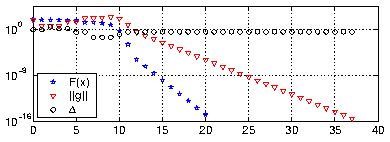
\includegraphics[width=0.72\linewidth]{assets/figures/fig-3-5.pdf}
\setcounter{figure}{4}
\caption{狗腿法用于 Powell 问题。}\label{fig:3.5}
\end{figure}

迭代在 $37$ 步后因梯度很小而停止，返回 $\mathbf{x}=[-2.41\cdot10^{-35},1.26\cdot10^{-9}]^{\T}$，这是 $\mathbf{x}^*=\mathbf{0}$ 的一个相当好的近似。与图~\ref{fig:3.3} 一样，可以看到最终是线性收敛（由 $\mathbf{J}(\mathbf{x}^*)$ 的奇异性引起），但明显快于 Marquardt 法。
\end{example}
